\documentclass{beamer}
\usetheme{Warsaw}
\setbeamertemplate{headline}{}

\usepackage{ae,lmodern}
\usepackage[english]{babel}
\usepackage[utf8]{inputenc}
\usepackage[T1]{fontenc}

\usepackage{caption}
\captionsetup[figure]{labelformat=empty}

\PassOptionsToPackage{usenames,dvipsnames}{xcolor}
\usepackage{xcolor,colortbl}
\definecolor{DarkGrey}{HTML}{222222}
\definecolor{DarkBlue}{HTML}{004BA9}
\definecolor{DarkRed}{HTML}{CC1111}
\definecolor{DarkGreen}{HTML}{117711}
\definecolor{DarkOrange}{HTML}{CC7000}
\definecolor{LightGrey}{HTML}{DDDDDD}
\definecolor{LightBlue}{HTML}{F0F8FF}
\definecolor{codegreen}{rgb}{0,0.6,0}
\definecolor{codepurple}{rgb}{0.58,0,0.82}

\usepackage[cache=false]{minted}
\setminted[bash]{
   bgcolor=LightBlue,
   breaklines, breakanywhere,
   frame=single,
   autogobble
}
\usemintedstyle[python]{native}
\setminted[python]{
   bgcolor=black,
   breaklines, breakanywhere,
   autogobble
}

\usepackage{listings}
\usepackage{lstautogobble}
\lstdefinestyle{bash}{
    backgroundcolor=\color{DarkGrey},   
    commentstyle=\color{codegreen},
    keywordstyle=\color{magenta},
    numberstyle=\tiny\color{DarkGrey},
    stringstyle=\color{codepurple},
    basicstyle=\ttfamily\tiny\color{LightGrey},
    escapeinside={\%*}{*)},
    breakatwhitespace=false,         
    breaklines=true,                 
    captionpos=b,                    
    keepspaces=true,                 
    numbers=left,                    
    numbersep=5pt,                  
    showspaces=false,                
    showstringspaces=false,
    showtabs=false,
    showlines=false,
    tabsize=2
}

\usepackage{tikz}
\usetikzlibrary{calc,decorations.pathreplacing,arrows,arrows.meta,shapes,patterns, positioning}
\newcommand\BigLength{14.6em}
\newcommand\Height{2em}
\newcommand\Sep{0.6em}
\newcommand\Center{\BigLength*1/2}
\newcommand\BigBox{\BigLength+\Sep}
\newcommand\HalfBox{\BigLength*1/2-\Sep*1/4}
\newcommand\HalfLength{\BigLength*1/2-\Sep*5/4}
\newcommand\CenterL{\BigLength*1/4-\Sep*1/8}
\newcommand\CenterR{\BigLength*3/4+\Sep*1/8}
\tikzstyle{layer}=[rectangle,thick,text centered,
                     minimum height=\Height,minimum width=\BigLength]
\tikzstyle{short}=[rectangle,thick,text centered,
                     minimum height=\Height,minimum width=\HalfLength]
\tikzstyle{dibox}=[rectangle,thick,semitransparent,
                     minimum height=(\Height+\Sep)*2,minimum width=\BigBox]
\tikzstyle{vmbox}=[rectangle,thick,semitransparent,
                     minimum height=(\Height+\Sep)*3,minimum width=\HalfBox]
\tikzstyle{ctbox}=[rectangle,thick,semitransparent,
                     minimum height=(\Height+\Sep)*2,minimum width=\HalfBox]
\tikzstyle{vebox}=[rectangle,thick,semitransparent,
                     minimum height=(\Height+\Sep)*1,minimum width=\HalfBox]

\usepackage{hyperref}
\usepackage{grffile}


\AtBeginSection[]
{
   \begin{frame}
      \tableofcontents[currentsection]
   \end{frame}
}

\AtBeginSubsection[]
{
   \begin{frame}
      \tableofcontents[currentsection, currentsubsection, sectionstyle=shaded]
   \end{frame}
}

%----------------------------------------------------------------------------------------
\title{Introduction to Data Science}
\subtitle{with Python}
%----------------------------------------------------------------------------------------
\author{Alexis Bogroff}
\date{\today}



\begin{document}

\begin{frame}
   \titlepage
\end{frame}

\begin{frame}\frametitle{Presenter}
   \begin{minipage}{0.3\linewidth}
      \centering
      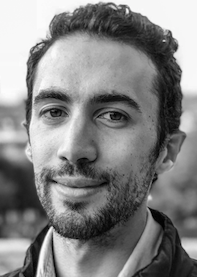
\includegraphics[width=0.6\textwidth]{../images/AlexisBogroff.png} \\
   \end{minipage}
   \begin{minipage}{0.6\linewidth}
      \noindent Alexis Bogroff \\
      Lecturer and Mentor in Data Science \\
      at Paris 1 Panthéon-Sorbonne, ESILV, Openclassrooms, EM-Lyon
   \end{minipage}
   \\[2ex]
   \visible<2->{\begin{itemize}
      \item 4 years Teaching Assistant and lecturer in VBA, Python for finance, SQL, Data Analysis and Data Science
      \item 9 months Researcher Assistant at Paris 1 Panthéon-Sorbonne within H2020 European Project
      \item 1 year Data Scientist at Pléiade Asset Management
   \end{itemize}}
   \hfill
\end{frame}

% \begin{frame}\frametitle{Overview}
%    \Large
%    \centering
%    Financial Engineering with Python Linux and Git \\[2ex]
%    \begin{minipage}{0.32\linewidth}
%       \includegraphics[width=0.8\textwidth]{../images/linux-1-logo-svg-vector.pdf}
%    \end{minipage}
%    \begin{minipage}{0.32\linewidth}
%       \includegraphics[width=0.8\textwidth]{../images/Git-logo.pdf}
%    \end{minipage}
%    \begin{minipage}{0.32\linewidth}
%       \includegraphics[width=0.9\textwidth]{../images/Python_logo_and_wordmark.pdf}
%    \end{minipage}
%    \pause
%    \\[3ex]
%    Free and everywhere stack \\
%    To find a job and be operational
% \end{frame}

% \begin{frame}\frametitle{Lecture Organisation}
%    \begin{itemize}[<+->]
%       \item Prerequisite:
%       \begin{enumerate}
%          \item Have a Linux environment working on your personal computer
%          \item[] (it can be WSL2 on Windows, Amazon EC2 for a distant solution)
%          \item Install Git
%          \item Install Python
%       \end{enumerate}
%       \vspace{2em}
%       \item Exam:
%       \begin{itemize}
%          \item Last QCM 1/2
%          \item Project 1/2
%       \end{itemize}
%    \end{itemize}
% \end{frame}


\begin{frame}
   \tableofcontents
\end{frame}

% =============================================================================
% =============================================================================
\section{Data Analysis}
% 3 Hours course (for Analysis and Pre-processing)
% =============================================================================
% =============================================================================


%------------------------------------------------------------------------------
\subsection{Measures}
%------------------------------------------------------------------------------

\begin{frame}\frametitle{Measures}
   \begin{itemize}
      \item Centrality:
      \begin{itemize}
         \item Average (mean)
         \item Median
      \end{itemize}
      \item Dispersion:
      \begin{itemize}
         \item Standard deviation (sqrt variance)
         \item Min-Max
         \item Interquartile Range (IQR)
      \end{itemize}

   \end{itemize}
\end{frame}

%------------------------------------------------------------------------------
\subsection{Patterns}
%------------------------------------------------------------------------------

\begin{frame}\frametitle{Patterns}
   \begin{itemize}
      \item Correlations
      \begin{itemize}
         \item Trend
         \item Saisonality
         \item Auto-correlation
      \end{itemize}
      \item Correlations with other variables:
      \begin{itemize}
         \item Linear
         \item Non-Linear
      \end{itemize}
   \end{itemize}
\end{frame}

\begin{frame}\frametitle{Correlation}
   \begin{itemize}
      \item Move repetitively in conjunction
      \item Methods
      \begin{itemize}
         \item Pearson
         \item Spearman (Rank)
      \end{itemize}
      \item Spurious correlation (ice cream, Eiffel Tower)
   \end{itemize}
\end{frame}


%------------------------------------------------------------------------------
\subsection{Statistical Tools}
%------------------------------------------------------------------------------

\subsubsection{Statistical Laws}

\begin{frame}\frametitle{Statistical Laws}
   \begin{itemize}
      \item Normal Law / Gauss Curve
      \begin{itemize}
         \item Totally resumed by mean and variance
         \item Constant mean (0 if centered) and variance (1 if reduced)
         \item Uncorrelated individuals
         \item Symetric (Skewness=0)
         \item Precise bell shape (Kurtosis=3)
      \end{itemize}

      \item Power Laws: multiplicative growth
      % TODO: insert graph examples of both distributions
      \item Examples:
      \begin{itemize}
         \item Normal: human age, size, weight, grades
         \item Power: lakes size, wealth
      \end{itemize}
   \end{itemize}
\end{frame}


\subsubsection{Statistical Tests}

\begin{frame}\frametitle{Statistical Tests}
   \begin{itemize}
      \item Intention: prevent sampling error
      \item Hypothesis (Normal Law)
      \item Examples:
      \begin{itemize}
         \item Normality test
         \item ANOVA
         \item Pearson's r
         \item Chi square
      \end{itemize}
         % TODO: review https://www.scribbr.com/statistics/statistical-tests/
   \end{itemize}
\end{frame}



% =============================================================================
% =============================================================================
\section{Data Pre-Processing}
% 3 Hours course (for Analysis and Pre-processing)
% =============================================================================
% =============================================================================


%------------------------------------------------------------------------------
\subsection{Data Management}
%------------------------------------------------------------------------------

\begin{frame}\frametitle{Data Management}
   \begin{itemize}
      \item Select variables
      \item Merge tables
      % TODO: add multiple code examples
   \end{itemize}
\end{frame}


%------------------------------------------------------------------------------
\subsection{Data Cleaning}
%------------------------------------------------------------------------------

\begin{frame}\frametitle{Data Cleaning}
   \begin{itemize}
      \item NaN Imputation
      \item Outliers
      % TODO: add multiple code examples
   \end{itemize}
\end{frame}


%------------------------------------------------------------------------------
\subsection{Feature Engineering}
%------------------------------------------------------------------------------

\begin{frame}\frametitle{Feature Engineering}
   \begin{itemize}
      \item Quantitative variables (numbers representing quantities): create groups
      \item Qualitative variables (categories): one-hot encode
      \item Filter
      % TODO: add multiple examples
   \end{itemize}
\end{frame}



\end{document}
